\chapter{TINJAUAN PUSTAKA}

Pada bab ini akan dibahas mengenai penelitian terkait tentang \emph{multi-tenancy}
dan teori dasar yang akan digunakan dalam penelitian.

\section{Hasil penelitian/perancangan terdahulu}

\subsection{Multi-tenancy in Cloud Computing}

Paper ini membahas mengenai definisi \emph{multi-tenancy} pada \emph{cloud computing}
dan bagaimana \emph{multi-tenancy} dapat diimplementasikan pada \emph{cloud computing} beserta
manfaat dan kekurangannya. \emph{Multi-tenancy} dapat berdampak positif pada perkembangan
\emph{cloud computing} karena dengan \emph{multi-tenancy}, sebuah server fisik dapat
dibagi kepada beberapa pengguna dengan teknologi virtualisasi. \emph{Multi-tenancy} memungkinkan
pemilik dari server fisik tersebut untuk mengurangi \emph{cost} dalam penyediaan
\emph{resources}.

Walaupun \emph{multi-tenancy} memiliki kelebihan tersebut,
\emph{multi-tenancy} pada \emph{cloud computing} juga memiliki tantangan dalam
implementasinya. Tantangan tersebut muncul karena \emph{multi-tenancy} memungkinkan
pengguna untuk berbagi \emph{resources} fisik yang sama. Hal tersebut dapat menimbulkan
tantangan dalam aspek keamanan.

Tantangan keamanan muncul karena pengguna yang berperan sebagai pelaku dan pengguna
yang menjadi korban berada pada satu server fisik yang sama. Kasus tersebut adalah
kasus yang unik dan hanya muncul di sistem yang menggunakan teknologi \emph{multi-tenancy}.
Contoh gambar perbedaan kasus antara \emph{multi-tenancy} dan tradisional terdapat pada
gambar \ref{fig:MultiTenancyCase}. Karena pelaku dan korban menggunakan \emph{resources}
fisik yang sama, proses mitigasi tradisional tidak dapat digunakan \parencite{6830928}.

\begin{figure} [H] \centering
  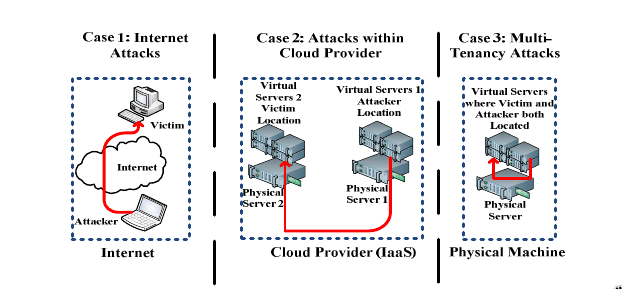
\includegraphics[scale=0.6]{gambar/multi-tenancy-case.png}
  \caption{Perbedaan kasus antara \emph{multi-tenancy} dan tradisional}
  \label{fig:MultiTenancyCase}
\end{figure}

\subsection{ViteraaS: Virtual Cluster as a Service}

Implementasi penggunaan \emph{virtual cluster} pada penelitian ini
berfokus pada pembagian banyak komputer fisik yang tergabung pada satu klaster
menjadi beberapa klaster virtual yang lebih kecil sesuai dengan kriteria yang diberikan oleh
pengguna seperti jumlah \emph{nodes} yang dibutuhkan.

Studi kasus yang digunakan pada penelitian ini adalah penggunaan sumber daya komputasi yang dimiliki oleh
universitas. Sumber daya komputasi pada universitas seperti PC dari lab dan server biasanya tidak
terutilisasi dengan baik (tidak begitu digunakan) pada saat malam dan libur semester. Namun, sumber daya
komputasi akan sangat banyak digunakan pada saat mendekati akhir semester dengan banyaknya tugas dan
ujian.

Dengan studi kasus yang sudah dijelaskan, penulis dari penelitian ini mengajukan sebuah \emph{virtual-cluster-as-a-service} bernama ViteraaS
yang digunakan untuk membuat \emph{virtual cluster} dari \emph{pool} sumber daya komputasi.
ViteraaS juga terintegrasi dengan infrastruktur yang sudah ada sebelumnya seperti \emph{Single Sign-On} (SSO).
Selain itu, ViteraaS juga mengutilisasi komponen lainnya seperti OpenNebula, sebuah \emph{tool} untuk mengatur infrastruktur virtual,
untuk membuat klaster \emph{virtual machine} secara dinamik \parencite{6133210}.

\subsection{A Multi-Tenant Framework for Cloud Container Services}

Kubernetes tidak memiliki fitur \emph{multi-tenancy} yang memadai. \emph{Multi-tenancy}
pada Kubernetes dapat dicapai melalui beberapa cara seperti menggunakan \emph{namespace}
untuk membagi \emph{resource} Kubernetes tiap pengguna dan menggunakan \emph{dedicated} klaster
untuk membagi \emph{permission} sehingga pengguna tidak dapat mengakses \emph{resource}
yang bukan miliknya. Namun, cara tersebut menimbulkan beberapa masalah seperti masalah
performa dan infrastruktur dari Kubernetes.

Penelitian ini membahas mengenai implementasi \emph{multi-tenancy} pada
Kubernetes dengan menggunakan \emph{framework} VirtualCluster. \emph{Framework}
VirtualCluster yang diajukan pada penelitian ini menyediakan isolasi pada \emph{control plane}
dan \emph{data plane} namun tetap berada di \emph{resources} fisik yang sama.

Implementasi dari \emph{framework} ini membuat setiap pengguna dalam klaster
memiliki \emph{control plane} dan \emph{data plane} tersendiri, sehingga dari
sisi pengguna, pengguna seperti memiliki sebuah klaster itu secara menyeluruh
dan tidak mengetahui pengguna lain yang menggunakan \emph{resources} fisik yang sama
\parencite{9546524}.

\section{Teori/Konsep Dasar}

\subsection{Kubernetes}

Kubernetes adalah sebuah platform manajemen aplikasi yang dikemas (\emph{containerized})
bersifat sumber terbuka. Kubernetes dibuat berdasarkan \emph{tool} internal
yang diciptakan oleh Google bernama Borg untuk mengelola layanan mereka dalam bentuk
\emph{container} \parencite{43438} kemudian beberapa pengembang Borg menciptakan
\emph{tool} serupa namun bersifat sumber terbuka yang kemudian diberi nama Kubernetes.

Kubernetes dapat mengelola jalannya aplikasi berbasis kontainer seperti membuat
aplikasi tersebut \emph{scalable} dengan cara menambah ataupun mengurangi kontainer
yang menjalankan aplikasi tersebut sesuai dengan kebutuhan pengguna, 

\subsection{Arsitektur Kubernetes}

Kubernetes mengumpulkan satu atau lebih mesin/server menjadi sebuah klaster. Klaster
pada Kubernetes adalah tempat dimana semua aplikasi, \emph{Jobs}, dan komponen Kubernetes
berjalan. Dalam satu klaster Kubernetes terdapat satu server atau satu kelompok server
yang berperan sebagai \emph{control plane} dan server sisanya menjadi \emph{worker node}.

Pada \emph{master node}, terdapat beberapa komponen yang mendukung kelangsungan
klaster seperti kube-apiserver, kube-controller-manager, kube-scheduler, dan etcd.
Sedangkan pada \emph{nodes} lainnya yang disebut sebagai \emph{worker node}
terdapat komponen kubelet dan kube-proxy \parencite{kubernetes-website-components}.
\emph{Worker node} bertugas untuk menjalankan \emph{Pod} yang berisi aplikasi
\emph{containerized}.

\subsubsection{Kubernetes Control Plane}

Kubernetes Control Plane adalah komponen yang bertugas untuk mengatur
klaster Kubernetes. \emph{Node} yang berperan sebagai Kubernetes Control Plane
membuat keputusan terhadap klaster sesuai dengan \emph{event} yang terjadi atau
konfigurasi yang diberikan. Interaksi dengan \emph{control plane} dapat dilakukan
melalui \emph{command line tool} dari Kubernetes yaitu kubectl.
Kubernetes Control Plane terdiri dari komponen-komponen
dalam membantu menjalankan tugas \emph{control plane} yaitu kube-apiserver,
etcd, kube-controller-manager, kube-scheduler, dan cloud-controller-manager.

\begin{enumerate}[itemsep=-0.2cm, topsep=-0.3cm]
  \item{Komponen kube-apiserver merupakan komponen yang
    bertujuan sebagai antarmuka untuk interaksi antar komponen dalam bentuk
    RESTful. Selain itu, kube-apiserver juga mengelola data untuk \emph{api objects}
    di dalam Kubernetes.
  }
  \item{Komponen etcd merupakan komponen yang digunakan
    oleh Kubernetes untuk menyimpan data dalam bentuk \emph{key-value}.
    Data tersebut kemudian digunakan sebagai konfigurasi klaster, proses
    \emph{service discovery}, dan data-data yang akan digunakan nantinya.
  }
  \item{Komponen kube-controller-manager adalah komponen yang
    mengawasi jalannya klaster. Komponen ini mengawasi \emph{shared state} dari
    klaster tersebut melalui kube-apiserver dan melakukan tindakan yang diperlukan
    agar mencapai \emph{state} yang diinginkan.
  }
  \item{Komponen kube-scheduler adalah komponen yang bertugas
    untuk menempatkan \emph{Pod} pada \emph{Node} yang sesuai. Komponen ini
    akan menentukan \emph{Node} yang sesuai dengan kriteria \emph{Pod} yang
    akan dijalankan.
  }
  \item{Komponen cloud-controller-manager merupakan komponen
    yang opsional dan digunakan oleh klaster Kubernetes untuk berinteraksi
    dengan API dari penyedia jasa \emph{cloud}. Komponen ini sebagai pemisah
    antara API dari penyedia jasa \emph{cloud} dengan API dari Kubernetes.
  }
\end{enumerate}

\subsubsection{Kubernetes Node}

Server lain selain Kubernetes Control Plane adalah \emph{worker node}
akan berperan sebagai tempat menjalankan \emph{Pod} yang berisi aplikasi
\emph{containerized}. \emph{Worker node} terdiri dari komponen kubelet, kube-proxy,
dan \emph{container runtime}.

\begin{enumerate}[itemsep=-0.2cm, topsep=-0.3cm]
  \item{Komponen kubelet adalah komponen agen yang berjalan pada
    setiap \emph{node} dalam klaster Kubernetes. Komponen ini bertugas untuk
    memastikan \emph{Pod} yang dijadwalkan pada \emph{Node} tersebut berjalan
    dengan baik.
  }
  \item{Komponen kube-proxy berjalan di setiap \emph{Node} pada
    klaster. Komponen ini bertugas untuk mengelola jaringan pada \emph{Node}.
    Jaringan tersebut digunakan untuk melakukan komunikasi dari dalam klaster
    maupun luar klaster menuju \emph{Pod}. Kube-proxy memastikan \emph{request}
    dikirimkan ke \emph{Pod}, lebih tepatnya \emph{container}, yang tepat serta bertanggung
    jawab atas jaringan tersebut sehingga dapat diakses dan diprediksi namun tetap terisolasi.
  }
  \item{Komponen \emph{container runtime} adalah komponen yang bertugas
    untuk mengatur \emph{container} pada \emph{node} tersebut karena pada dasarnya setiap
    \emph{Job} atau aplikasi yang dibuat pada klaster akan dijalankan di dalam \emph{container}.
    Kubernetes mendukung beberapa \emph{container runtime} yang ada yaitu Docker, containerd, dan
    \emph{container} yang mengimplementasikan Kubernetes Container Runtime Interface (CRI).
  }
\end{enumerate}

\subsection{Objek pada Kubernetes}

Kubernetes memiliki beberapa objek yang digunakan untuk mengatur jalannya
klaster. Objek pada Kubernetes merupakan entitas persisten yang ada pada sistem
Kubernetes. 

\subsubsection{\emph{Pod}}

\emph{Pod} adalah unit terkecil yang dapat dibuat dalam Kubernetes. Aplikasi
\emph{containerized} dijalankan di dalam \emph{Pod}. \emph{Pod} pada Kubernetes
dapat berisi satu atau lebih \emph{container} yang saling berbagi \emph{network}
dan \emph{storage}. Konfigurasi \emph{Pod} dapat diatur melalui sebuah konfigurasi
Podspec yang memiliki ekstensi .yaml.

\subsubsection{\emph{Job}}

\emph{Job} merupakan beban kerja pada Kubernetes. \emph{Job} akan menciptakan satu atau
lebih \emph{Pod} untuk menyelesaikan tugas tersebut. \emph{Pod} yang diciptakan untuk menyelesaikan
\emph{Job} akan berhenti jika \emph{Job} yang dilakukan sudah selesai. Jika \emph{Pod}
berhenti namun \emph{Job} terkait masih belum selesai, \emph{Job} akan menciptakan \emph{Pod}
baru untuk melanjutkan \emph{Job} tersebut. \emph{Job} dapat menciptakan lebih dari satu
\emph{Pod} untuk menyelesaikan tugas tersebut secara paralel.

\subsubsection{\emph{Replication Controllers} dan \emph{ReplicaSet}}

\emph{Replication Controllers} adalah objek yang mendefinisikan sebuah \emph{pod template}
dan parameter kontrol untuk melakukan \emph{scaling} secara horizontal dengan menambahkan
atau mengurangi jumlah \emph{Pod} yang sedang berjalan. \emph{Replication Controllers}
bertanggung jawab untuk memastikan jumlah \emph{Pod} yang ada pada sebuah klaster
sesuai dengan jumlah \emph{Pod} yang didefinisikan di awal oleh pengguna.

\emph{ReplicaSet} merupakan versi lebih baru dari \emph{Replication Controllers} yang
bertujuan untuk mengelola kumpulan \emph{Pod} yang stabil dan sedang berjalan. \emph{ReplicaSet}
dapat melakukan mekanisme \emph{self-healing} dimana \emph{ReplicaSet} akan menjalankan
kembali secara otomatis \emph{Pod} yang mengalami kegagalan saat sedang berjalan. \emph{ReplicaSet}
juga dapat menambahkan atau mengurangi jumlah \emph{Pod} sama seperti \emph{Replication Controllers}.

\subsubsection{\emph{Service}}

\emph{Service} pada Kubernetes merupakan abstraksi dari \emph{Pod} yang bertugas untuk
menyediakan sebuah alamat IP dan DNS untuk mengakses \emph{Pod} tersebut. \emph{Service}
merupakan objek yang mengimplementasikan arsitektur REST. \emph{Service} memiliki beberapa tipe,
yaitu ClusterIP, NodePort, LoadBalancer, dan ExternalName.

\begin{enumerate}[itemsep=-0.2cm, topsep=-0.3cm]
  \item{ClusterIP adalah tipe \emph{Service} yang mengekspos \emph{Service}
      pada IP internal klaster. Dengan adanya ClusterIP, \emph{Service} hanya bisa
      diakses dari dalam klaster.
    }
  \item{NodePort adalah tipe \emph{Service} yang mengekspos \emph{Service}
      pada alamat IP dan \emph{port} statik setiap \emph{node}. Dengan tipe ini, \emph{Service}
      dapat diakses dari luar dengan melakukan \emph{request} pada NodeIP dan NodePort.
    }
  \item{LoadBalancer adalah tipe \emph{Service} yang mengekspos \emph{Service} ke eksternal klaster
      dengan menggunakan \emph{load balancer}. Kubernetes tidak menyediakan \emph{load balancer}
      secara \emph{default}.
    }
  \item{ExternalName adalah tipe \emph{service} yang memetakan \emph{service} dengan sebuah
      \emph{external name} dengan cara mengembalikan CNAME bersama dengan nilainya.
    }
\end{enumerate}

\subsubsection{\emph{Horizontal Pod Autoscaler}}

\emph{Horizontal Pod Autoscaler} adalah layanan dari Kubernetes yang memungkinkan
\emph{scaling} jumlah \emph{Pod} yang ada pada \emph{Replication Controller} dan \emph{ReplicaSet} berdasarkan
metrik tertentu yang bisa ditetapkan seperti penggunaan CPU dan memori secara otomatis.
\emph{Horizontal Pod Autoscaler} diimplementasikan dalam bentuk sumber daya pada Kubernetes
API dan \emph{controller}. \emph{Controller} tersebut secara periodik akan mengatur
jumlah dari replika pada \emph{Replication Controller} sesuai dengan metrik penggunaan
sumber daya dan target yang didefinisikan oleh pengguna.
Cara kerja dari \emph{Horizontal Pod Autoscaler} ditunjukkan pada gambar \ref{fig:HorizontalPodAutoscalling}

\emph{Horizontal Pod Autoscaler} menggunakan perbandingan dari metrik yang diinginkan
dengan metrik keadaan saat ini. Hasil perbandingan tersebut akan digunakan sebagai penentuan
jumlah replika yang akan dibuat. Persamaan untuk \emph{Horizontal Pod Autoscaler} dapat
dilihat pada persamaan \ref{eq:hpaAlgorithm}.

\begin{equation}
  desiredReplicas = ceil [ currentReplicas \times \left( \frac{currentMetricValue}{desiredMetricValue} \right) ]
  \label{eq:hpaAlgorithm}
\end{equation}

Nilai dari \emph{currentMetricValue} juga dapat dihitung berdasarkan rata-rata nilai
sasaran pada seluruh \emph{Pod} tujuan apabila parameter \emph{targetAverageValue} atau
\emph{targetAverageUtilization} ditentukan.

\begin{figure} [H] \centering
  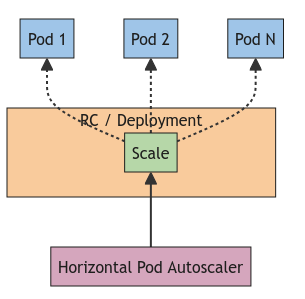
\includegraphics[scale=0.6]{gambar/horizontal_pod_autoscalling_figure.png}
  \caption{Horizontal Pod Autoscaler Kubernetes \parencite{kubernetes-website-hpa}}
  \label{fig:HorizontalPodAutoscalling}
\end{figure}

\subsubsection{\emph{Kubernetes Cluster Autoscaler}}

\emph{Kubernetes Cluster Autoscaler} digunakan untuk melakukan \emph{autoscaling}
ukurang dari suatu klaster Kubernetes secara otomatis. Berbeda dengan \emph{autoscaling}
yang dilakukan oleh \emph{Horizontal Pod Autoscaler} dan \emph{Vertical Pod Autoscaler} yang
melakukan \emph{scaling} pada \emph{container} dan \emph{Node}, \emph{Kubernetes Cluster Autoscaler}
melakukan \emph{scaling} pada infrastruktur dengan cara menambahkan atau mengurangi jumlah
\emph{Node} pada suatu klaster.

\subsubsection{\emph{Namespace}}

Kubernetes menyediakan fitur isolasi \emph{resources} dalam satu klaster dengan
menggunakan \emph{namespace}. \emph{Namespace} digunakan dalam \emph{environment}
Kubernetes yang memiliki beberapa pengguna atau tim dalam satu klaster. \emph{Namespace}
menyediakan \emph{scope} untuk nama \emph{resources}. Nama \emph{resources} harus unik
dalam satu \emph{namespace} namun tidak harus unik antar \emph{namespace}. \emph{Namespace}
tidak dapat dibagi secara \emph{nested} (menggunakan \emph{namespace} dalam \emph{namespace})
dan tiap \emph{resources} hanya dapat berada dalam satu \emph{namespace}.

Secara \emph{default}, Kubernetes memiliki beberapa \emph{namespace} yang sudah
tersedia, yaitu \emph{default}, \emph{kube-node-lease}, \emph{kube-public}, dan \emph{kube-system}.

\begin{enumerate}[itemsep=-0.2cm, topsep=-0.3cm]
  \item{\emph{Namespace default} adalah \emph{namespace} yang dibuat secara otomatis
      pada saat membuat klaster Kubernetes sehingga pengguna klaster dapat langsung
      menggunakan klaster tanpa harus membuat \emph{namespace} terlebih dahulu.
    }
  \item{\emph{Namespace kube-node-lease} adalah \emph{namespace} yang berisi objek \emph{Lease}
      Kubernetes pada setiap \emph{Node}. Objek \emph{Lease} digunakan oleh kubelet untuk
      mengirim \emph{heartbeat} untuk mendeteksi apakah \emph{Node} tersebut masih hidup atau tidak.
    }
  \item{\emph{Namespace kube-public} adalah \emph{namespace} yang dapat diakses oleh semua
      klien dan biasanya berisi informasi dari penggunaan klaster.
    }
  \item{\emph{Namespace kube-system} adalah \emph{namespace} yang berisi objek yang diciptakan
      oleh Kubernetes.
    }
\end{enumerate}

\subsection{Menambah \emph{worker node} pada klaster Kubernetes}

Kubernetes memiliki protokol untuk menambahkan \emph{worker nodes} ke dalam klaster Kubernetes.
Ketika sebuah \emph{worker node} ingin bergabung ke klaster Kubernetes, diperlukan hubungan
dua arah antara \emph{worker node} dan klaster. Hubungan ini dapat dibagi menjadi dua proses, yaitu
proses \emph{discovery} (\emph{node} memercayai klaster) dan \emph{bootstrap} TLS (klaster memercayai \emph{node}) \parencite{kubernetes-website-adding-linux-node}.

Terdapat 2 skema utama dalam proses \emph{discovery}. Skema pertama yaitu menggunakan token bersama beserta
alamat IP dari API server. Skema kedua adalah menyediakan sebuah \emph{file} yang merupakan
\emph{subset} dari standar konfigurasi kubeconfig yang berisi informasi yang diperlukan oleh
\emph{node} untuk bergabung ke klaster.

Untuk mempermudah proses tersebut, Kubernetes memiliki \emph{tool} untuk menambahkan \emph{worker node} ke dalam sebuah klaster
baik itu \emph{worker node} Linux \emph{operating system} atau \emph{worker node} Windows \emph{operating system}.
\emph{Tool} tersebut adalah kubeadm. Kubeadm merupakan \emph{tool} berbasis \emph{command line} untuk mengatur administrasi dari sebuah klaster
Kubernetes. Kubeadm dapat membuat sebuah klaster serta menggabungkan sebuah \emph{node} ke dalam klaster.

\subsection{\emph{Multi-tenant}}

\emph{Multi-tenant} yang berarti banyak penyewa adalah konsep dimana sebuah sistem
atau \emph{resources} dapat digunakan oleh lebih dari satu penyewa atau pengguna. Dalam
konteks Kubernetes, \emph{multi-tenancy} berarti sebuah lingkungan Kubernetes dan \emph{resources}-nya
dapat digunakan oleh lebih dari satu pengguna \parencite{oliva_multi-tenancy_2024}. Contoh gambar
implementasi \emph{multi-tenancy} pada Kubernetes terdapat pada gambar \ref{fig:KubernetesMultiTenancy}

\begin{figure} [H] \centering
  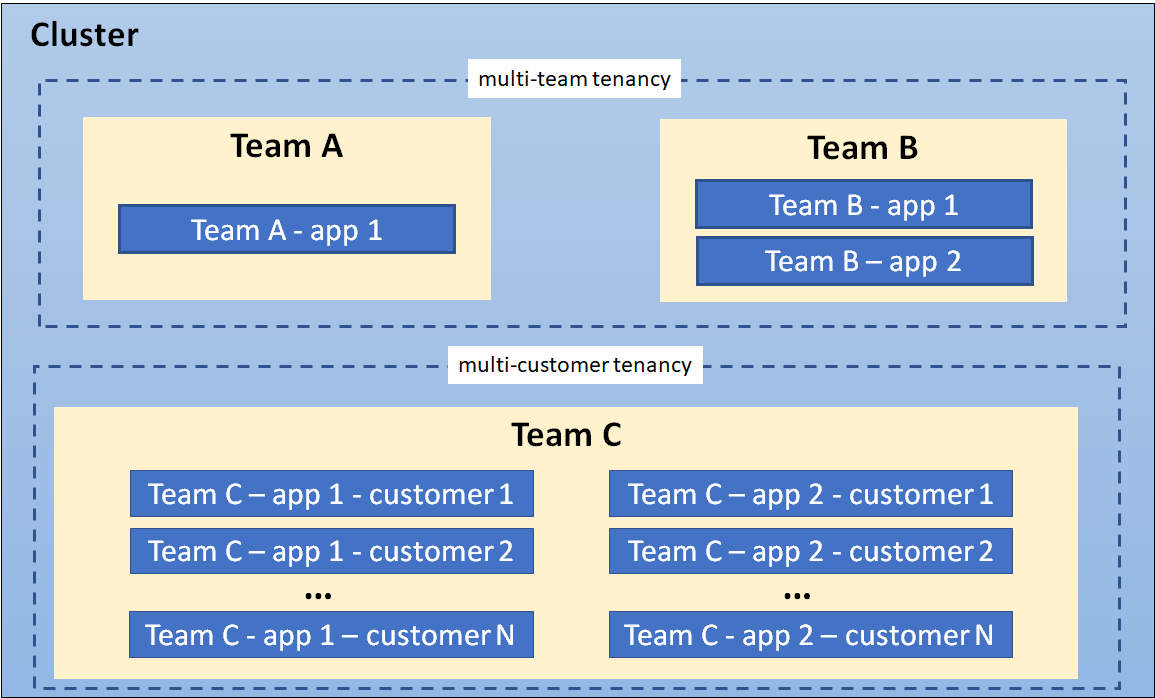
\includegraphics[scale=0.7]{gambar/multi-tenancy.png}
  \caption{\emph{Multi-tenancy} pada Kubernetes \parencite{kubernetes-website-multi-tenancy}}
  \label{fig:KubernetesMultiTenancy}
\end{figure}

Pada gambar di atas, implementasi \emph{multi-tenancy} pada Kubernetes
membagi klaster berdasarkan pengguna dari klaster hasil pembagian, yaitu pembagian
klaster untuk tim dalam projek dan pelanggan dari projek.

\emph{Multi-tenancy} juga dapat didefinisikan pada persamaan \ref{eq:multiTenancyEquation}

\begin{equation}
  \textit{Virtualization} + \textit{ResourceSharing} = \textit{Multi-Tenancy}
  \label{eq:multiTenancyEquation}
\end{equation}

Berdasarkan persamaan di atas, \emph{multi-tenancy} dapat dicapai dengan penggabungan antara
teknologi virtualisasi dan \emph{resource sharing} \parencite{6830928}.

Sistem atau \emph{resources} yang memiliki sifat \emph{multi-tenancy} harus memiliki
mekanisme isolasi \emph{resources} untuk setiap pengguna dalam sistem. Hal tersebut
diperlukan agar satu pengguna tidak memiliki akses terhadap \emph{resources} dari
pengguna lainnya. Isolasi \emph{multi-tenancy} pada Kubernetes terdiri dari beberapa
jenis, yaitu isolasi pada tingkat \emph{namespace}

% NOTE: this needs more explanation
\subsection{\emph{Virtual cluster}}

\emph{Virtual cluster} adalah klaster yang dibuat di atas klaster yang tersedia.
\emph{Virtual cluster} dapat digunakan untuk membagi klaster yang ada menjadi beberapa
klaster yang lebih kecil. Dengan menggunakan \emph{virtual cluster}, sebuah klaster
dapat digunakan oleh beberapa pengguna yang menggunakan klaster tersebut dengan
menggunakan \emph{virtual cluster} yang berbeda-beda dalam satu waktu. Dengan
menggunakan klaster yang berbeda, maka isolasi \emph{resources} antar pengguna
dapat terpenuhi.
